\section{Overview}
 
\begin{figure}[ht!]
  \centering
  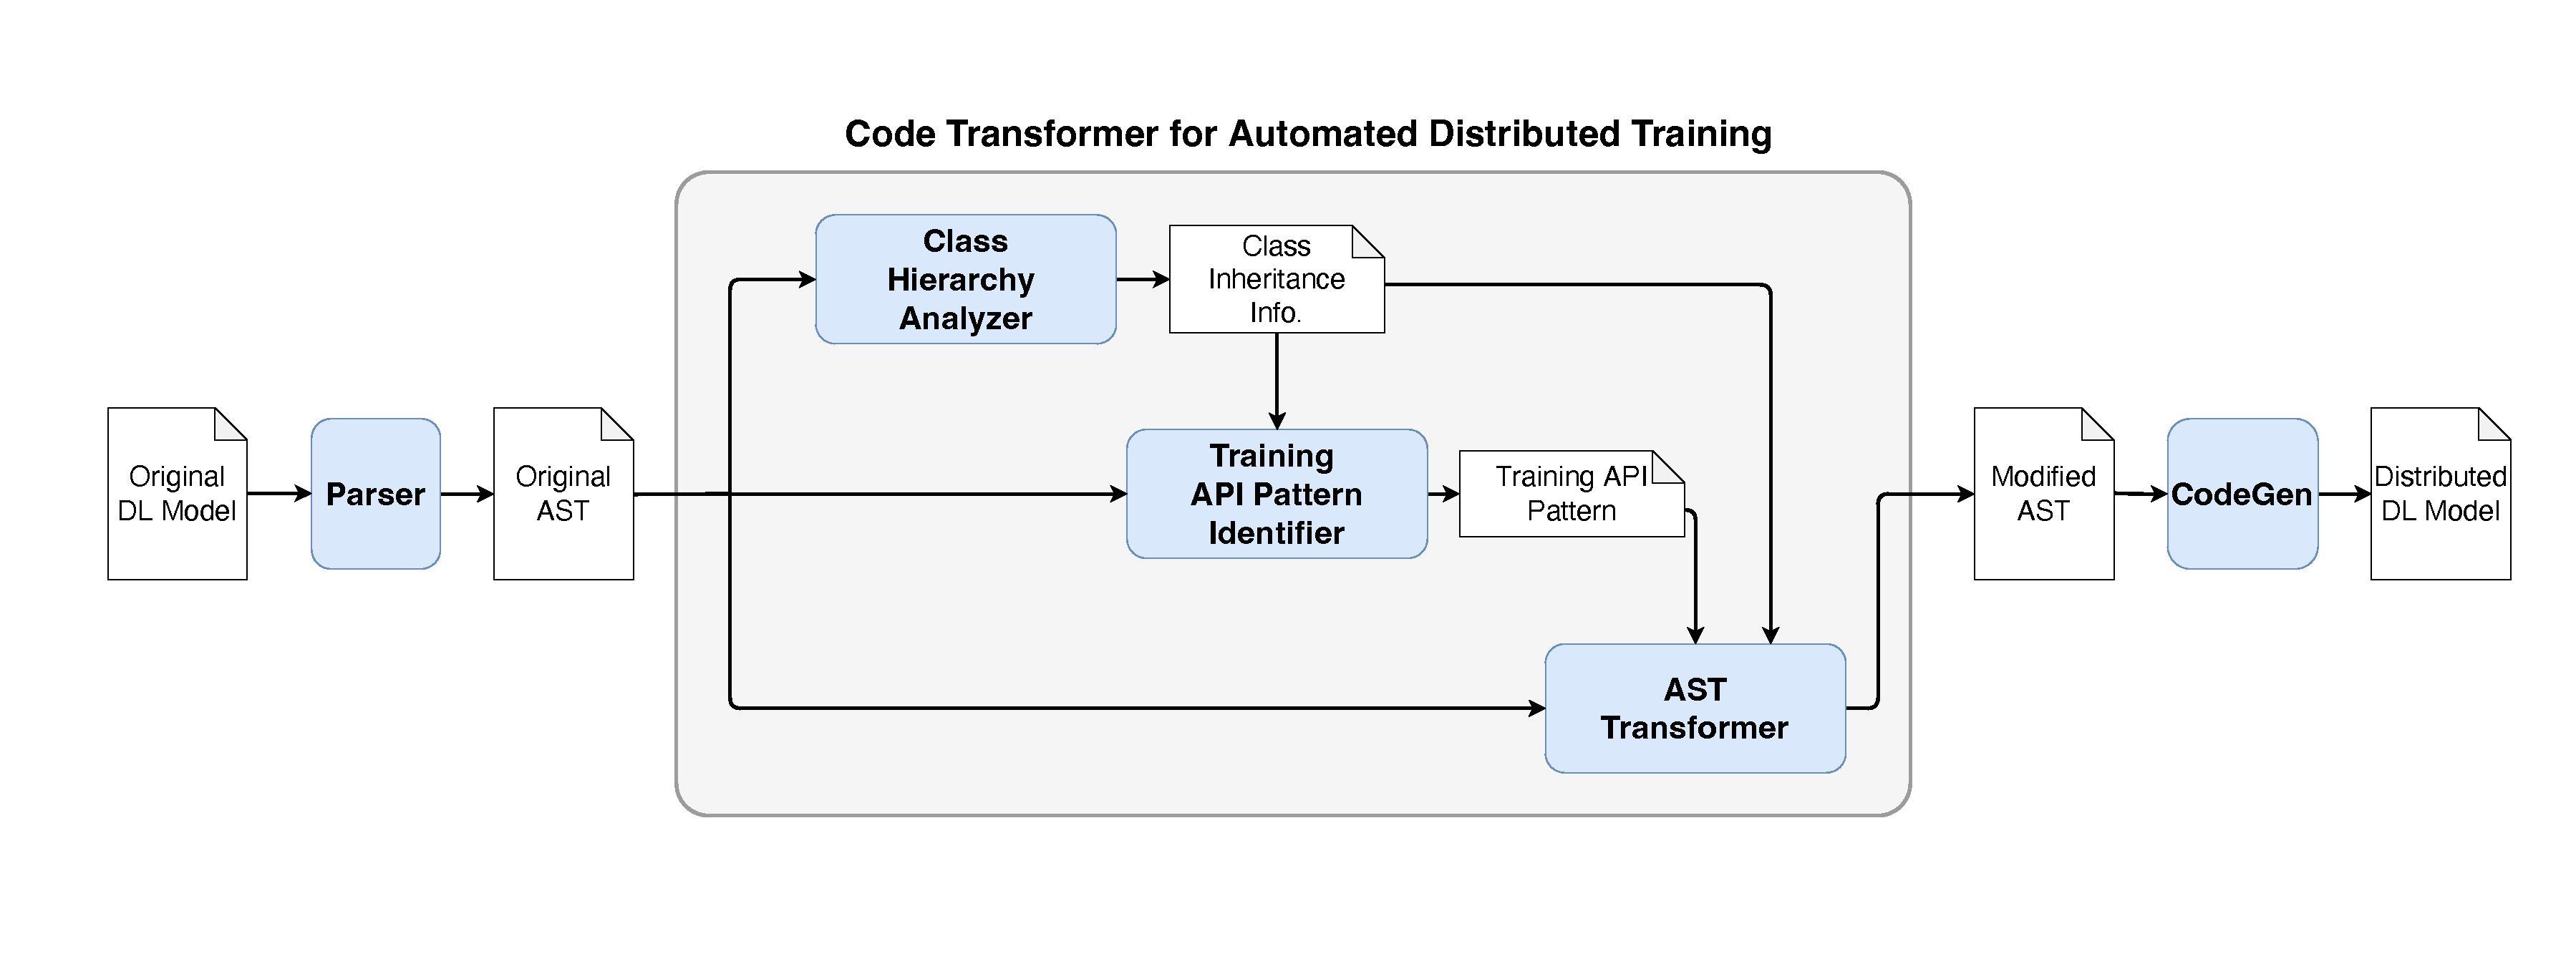
\includegraphics[width=\textwidth]{overview_diagram.pdf}
  \caption{Overall structure of the 
  automated transformation for distributed training}
  \label{sysarch}
\end{figure}

% main topic sentence for each paragraph

% 우리는 코드 변환을 기반을 기존의 모델을 자동으로 분산화하는 기법을 제안한다.
This paper proposes an automated code transformation method that rewrites
TensorFlow DL models to the distributed versions with Horovod.
As discussed in the previous section, distributed training with the Horovod
library requires model engineers to understand the Horovod library and rewrite
model code manually.
To alleviate this burden, our proposed method utilizes static analysis and code
transformation techniques to rewrite TensorFlow DL model code automatically
based on our formal transformation rules.
% to simplify the process of distributing DL models.

%We propose the code transformation-based approach for automated distributed
%training of TensorFlow DL models.
%As explained in the previous section, distributing TensorFlow DL models with
%Horovod library requires adding and editing the original models.
%Currently, the developers must fully understand the model codes and manually
%rewrite them.
%This also includes understanding the Horovod library usage by reading the
%library documentation and code exmaples.
%To ease the burden of the rewriting process, we utilize the code transformation
%technique to automatically rewrite the input TensorFlow model code with Horovod
%library.

Figure \ref{sysarch} illustrates the overview of our automated code
transformation approach for distributed training of DL models with Horovod.
Our approach first parses a given model into Abstract Syntax Trees
(ASTs) to analyze and modify the model code mechanically.
In order to define the code transformation rules for the distributed training
of TensorFlow DL models, we manually inspected the Horovod library
documentation and code examples. 
Through this analysis, we found that different transformation rules are
necessary for TensorFlow models depending on the specific TensorFlow APIs used
in the models.
Thus, we defined four \textit{training API patterns} that represent common code
patterns of TensorFlow APIs that appear in TensorFlow DL models.
The \cha~analyzes the ASTs and extracts the class
inheritance information relations between TensorFlow built-in and
user-defined classes.
Using the inheritance information, the \tapi~identifies the training API
pattern of the input model.  Then, the \atran~selects the appropriate
transformation rules based on the identified training API pattern and applies
the rules to the model's ASTs. 
The modified ASTs are then finally converted back into a TensorFlow DL
model, and the model can now train on multiple GPUs with the support of
the Horovod library.

%The modified ASTs are finally converted into Python codes to return
%the distriubted model as an output.

% 기존의 모델에 적용하는 코드 변환 규칙을 정의하기 위해 horovod 라이브러리 문서와
% 코드 예제를 검토했다. 그 결과로 TF 모델을 4가지로 분류하고 각 분류에 맞는
% 변환 규칙을 정의할 수 있었다.

%To define the code transformation rule for distributed training of 
%TensorFlow DL models,
%we manually inspected the Horovod library documentation and code examples.
%In this end, we identified four categories of TensorFlow DL models.
%We define four \textit{training API patterns}, which are common code patterns of 
%TensorFlow APIs appearing in each category of the TensorFlow DL models.
%To categorize the TensorFlow DL models into one of the four patterns, 
%we implemented the \textit{training API pattern identifier}. 
%In this process, we identified that the training API pattern identifier 
%must know the class inheritance relationship between TensorFlow library 
%classes and user-defined classes.
%To solve this problem, we also implemented the \textit{class hierarchy analyzer}
%to retrieve the class inheritance information of the TensorFlow DL model.



% 우리 기법은 입력으로 주어진 TF 모델에서 먼저 API 패턴을 인식하고
% 해당 패턴에 맞는 코드 변환 규칙을 적용하는 방식으로 작동한다.
% 이를 위해 설계한 우리 기법의 overview는 피규어와 같다...
%Figure \ref{sysarch} illustrates the overview of our approach.
%Given the single-GPU model as an input, our approach parses the model codes
%into ASTs in order to mechanically analyze and modify them.
%We first analyze the class hierarchy of the input TensorFlow model
%to produce the class inheritance information.
%Then the training API pattern identifier uses the inheritance information to
%identify the training API pattern of the input model.
%Finally, the AST transformer selects the correct transformation rule
%according to the training API pattern then apply the rule to the model ASTs.
%The modified ASTs are finally converted into Python codes to return
%the distriubted model as an output.

The subsequent sections provide detailed explanations of each component of our
proposed approach. 
Section \ref{sec:cha} describes the necessity of the class hierarchy analysis
for our approach.
Section \ref{sec:pattern} explains the concept of training API patterns and the
implementation of the \tapi.
Finally, Section \ref{sec:trans} provides a detailed description of the code
transformation process for each identified training API pattern, including the
formalization of the corresponding transformation rules.
